\documentclass[10pt,a4paper,ngerman]{article}

% adjust the page sizes to your likings
\usepackage[left=3.5cm,right=3.5cm,top=2.5cm,bottom=2.5cm]{geometry}
\usepackage[utf8]{inputenc}
\usepackage[ngerman]{babel}
\usepackage[T1]{fontenc} % allow west-european symbols (also umlauts: ä, ö, ü)
\usepackage{csquotes} % for \enquote{}
\usepackage{float} % for floating images
\usepackage[bottom]{footmisc} % keep footnotes at the bottom of the page
\usepackage{setspace} % to have the \setstretch{baselinestrech} command available
\usepackage{ragged2e} % text alignment
\usepackage[parfill]{parskip} % no indentation for paragraphs, instead add spacing
\usepackage{pdfpages} %for including pdf
\usepackage{rotating}
\usepackage{tikz-cd}
\usepackage{subcaption}
\usepackage{graphicx}
\usepackage{tabularx}
\usepackage{booktabs}
\usepackage{multirow}

% Rotate pages 90°, e.g. for wide tables.
% https://tex.stackexchange.com/a/25371/249769
\usepackage{pdflscape}
% scale whole boxes, e.g. tables
% https://tex.stackexchange.com/a/121198/249769
\usepackage{adjustbox}


% Easy tables, e.g. for coloring columns as seen here.
% https://tex.stackexchange.com/a/613906/
% \usepackage{tabularray}

% Graphics & Color
\usepackage{xcolor}
\definecolor{heidelberg-red}{HTML}{E50A37}
\usepackage{graphicx}

% Math & Physics
\usepackage{amsmath}
\usepackage{amsfonts}
\usepackage{amsthm}
\usepackage{amssymb}
\usepackage{bm}
\usepackage{cancel}

% Chemics
\usepackage{chemformula}
\setchemformula{circled=all}

\usepackage{witharrows} % http://mirrors.ibiblio.org/CTAN/macros/generic/witharrows/witharrows.pdf
\usepackage{nicefrac} % usage: \nicefrac{nominator}{denominator}
\usepackage{physics}
\usepackage{siunitx}
\sisetup{
	locale=US,
	group-separator={,},
	group-digits=integer,
	quotient-mode=fraction,per-mode=symbol}
\usepackage{empheq} % boxed equations: https://trucastuces.wordpress.com/2012/10/10/boxed-equations-in-latex/

\usepackage{lmodern}
\usepackage{fancyhdr}
\usepackage{enumerate}
% we use the option hidelinks here to avoid ugly borders around clickable items, e.g. links and cross-references
\usepackage{hyperref} % clickable links
\hypersetup{
	colorlinks = true,
	linkcolor={red!50!black}, % Color of internal links
	% citecolor={blue!50!black}, % Color of citations
	urlcolor={blue!80!black} % Color for external hyperlinks
}
\usepackage{todonotes}
\setlength {\marginparwidth }{2cm}      % margin for todo notes
\usepackage[nameinlink]{cleveref}

\let\qty\SI % see "bug" (warning) in https://tex.stackexchange.com/a/628184

% Enumerations
\usepackage{enumitem}
% Enumerate lists as a) b) instead of 1. 2.
\setenumerate[0]{label=\textbf{\alph*)}}
% remove indentation of enumerate environment
\setlist{leftmargin=*}
% for convenience
% usage: \q{I am citing} in order to get "I am citing"
\newcommand{\q}[1]{\enquote{#1}}

\newcommand{\set}[1]{\ensuremath{\{\,#1\,\}}}
\newcommand*{\coloniff}{\ratio\Leftrightarrow}
\newcommand*{\colonLeftrightarrow}{\ratio\Leftrightarrow}
\renewcommand{\implies}{\Rightarrow}
\renewcommand{\impliedby}{\Leftarrow}
\renewcommand{\iff}{\Leftrightarrow}
\newcommand{\definedAs}{\ratio\Leftrightarrow}
\newcommand{\perc}[1]{\ensuremath{\qty{#1}{\percent}}}
\newcommand{\solution}[1]{\ensuremath{\underline{\underline{#1}}}}
\newcommand{\determ}{\operatorname{det}}
\newcommand{\R}{\mathbb{R}}

% German specific
\newcommand{\zB}{z.\,B. }
\newcommand{\dash}{d.\,h. }

% Text over equal sign, e.g. to indicate that a specific definition was used
% usage: \eqdef{text over equal sign}
% https://tex.stackexchange.com/a/74132
\newcommand{\eqdef}[1]{\mathrel{\overset{\makebox[0pt]{\mbox{\normalfont\tiny\sffamily #1}}}{=}}}
\newcommand{\impliesdef}[1]{\mathrel{\overset{\makebox[0pt]{\mbox{\normalfont\tiny\sffamily #1}}}{\implies}}}
% https://tex.stackexchange.com/questions/9466/color-underline-a-formula
\newcommand{\mline}[2][red]{\color{#1}\underline{{\color{black}#2}}\color{black}}

% Math environments
\newenvironment{eqarrows}{
	\begin{equation}
		\begin{WithArrows}
		}{%
		\end{WithArrows}
	\end{equation}
	\ignorespacesafterend
}
\newenvironment{eqarrows*}[1][]{
	\begin{equation*}
		\begin{WithArrows}[#1]
		}{%
		\end{WithArrows}
	\end{equation*}
	\ignorespacesafterend
}
\newenvironment{eqboxed}{
	% https://tex.stackexchange.com/questions/419132/newenvironment-with-empheq-inside-tcolorbox
	\empheq[box=\fbox]{align}
	}{%
	\endempheq%
	\ignorespacesafterend
}
\newenvironment{eqboxed*}{
	% https://tex.stackexchange.com/questions/419132/newenvironment-with-empheq-inside-tcolorbox
	\empheq[box=\fbox]{align*}
	}{%
	\endempheq%
	\ignorespacesafterend
}

% Other math stuff
% vector with prime symbol
\newcommand{\vecp}[1]{\ensuremath{\vec{#1}^{\,\prime}}}
\newcommand{\dvecp}[1]{\ensuremath{\dvec{#1}^{\,\prime}}}
\newcommand{\ddvecp}[1]{\ensuremath{\ddvec{#1}^{\,\prime}}}
% vector prime with subscript
\newcommand{\vecps}[2]{\ensuremath{\vec{#1}^{\,\prime}_{\!#2}}}

% copied from https://tex.stackexchange.com/a/44071/249769
% Macro \xvec
\makeatletter
\newlength\xvec@height%
\newlength\xvec@depth%
\newlength\xvec@width%
\newcommand{\xvec}[2][]{%
	\ifmmode%
	\settoheight{\xvec@height}{$#2$}%
	\settodepth{\xvec@depth}{$#2$}%
	\settowidth{\xvec@width}{$#2$}%
	\else%
	\settoheight{\xvec@height}{#2}%
	\settodepth{\xvec@depth}{#2}%
	\settowidth{\xvec@width}{#2}%
	\fi%
	\def\xvec@arg{#1}%
	\def\xvec@dd{:}%
	\def\xvec@d{.}%
	\raisebox{.2ex}{\raisebox{\xvec@height}{\rlap{%
				\kern.05em%  (Because left edge of drawing is at .05em)
				\begin{tikzpicture}[scale=1]
					\pgfsetroundcap
					\draw (.05em,0)--(\xvec@width-.05em,0);
					\draw (\xvec@width-.05em,0)--(\xvec@width-.15em, .075em);
					\draw (\xvec@width-.05em,0)--(\xvec@width-.15em,-.075em);
					\ifx\xvec@arg\xvec@d%
					\fill(\xvec@width*.45,.5ex) circle (.5pt);%
					\else\ifx\xvec@arg\xvec@dd%
					\fill(\xvec@width*.30,.5ex) circle (.5pt);%
					\fill(\xvec@width*.65,.5ex) circle (.5pt);%
					\fi\fi%
				\end{tikzpicture}%
	}}}%
	#2%
}
\makeatother

% --- Override \vec with an invocation of \xvec.
\let\stdvec\vec
\let\ovec\vec
\renewcommand{\vec}[1]{\xvec[]{#1}}
% --- Define \dvec and \ddvec for dotted and double-dotted vectors.
\newcommand{\dvec}[1]{\xvec[.]{#1}}
\newcommand{\ddvec}[1]{\xvec[:]{#1}}


% Meta values
\newcommand{\subject}{Schwankungen von Bäumen}
\newcommand{\subjectshort}{Bäume}
\newcommand{\experimentnumber}{42}
\newcommand{\experiment}{Experiment \experimentnumber}
\newcommand{\advisor}{Betreuer: ABC}
\newcommand{\authors}{Splines}
\newcommand{\experimentdate}{05.07.1687}
\newcommand{\group}{Newton'sche Vormittagsgruppe}

% Header
\pagestyle{fancy}
\lhead{\experimentnumber: \subjectshort}
\rhead{\rightmark}

\setstretch{1.25}
\begin{document}
\setlength{\abovedisplayskip}{0.2em}
%\setlength{\belowdisplayskip}{0pt}
%\setlength{\abovedisplayshortskip}{0pt}
%\setlength{\belowdisplayshortskip}{0pt}

\thispagestyle{plain} % empty header, footer contains page number

% smaller top margin on first page
\vspace*{-2cm}

\begin{FlushLeft}
	\LARGE \textbf{\subject}\\
	\large \experiment\\
	
	\normalsize \advisor\\
	\authors\\
	
	\experimentdate, \group
	\hfill
	
	\vspace{3mm}
	
	\textcolor{heidelberg-red}{\rule{\linewidth}{1mm}}
\end{FlushLeft}

% Content
\tableofcontents
\setcounter{section}{0}
\pagebreak
\section{Einführung}

Dies ist das wichtigste Forschungsgebiet in der Physik.


\subsection{Reibungskräfte}

\autoref{fig:forces-on-rolling-body} zeigt, wie ein Baumstamm eine schiefene Ebene (Winkel $\varphi$) herunterollt. Die Reibungskraft $F_R$ hängt dabei vom Alter und damit von den Anzahl an Baumringen ab. In diesem Fall schließt der Baumstamm mindestens 2 Karokästchen ein, was einem Alter von 60 Jahren entspricht.

\begin{figure}[h]
    \centering
    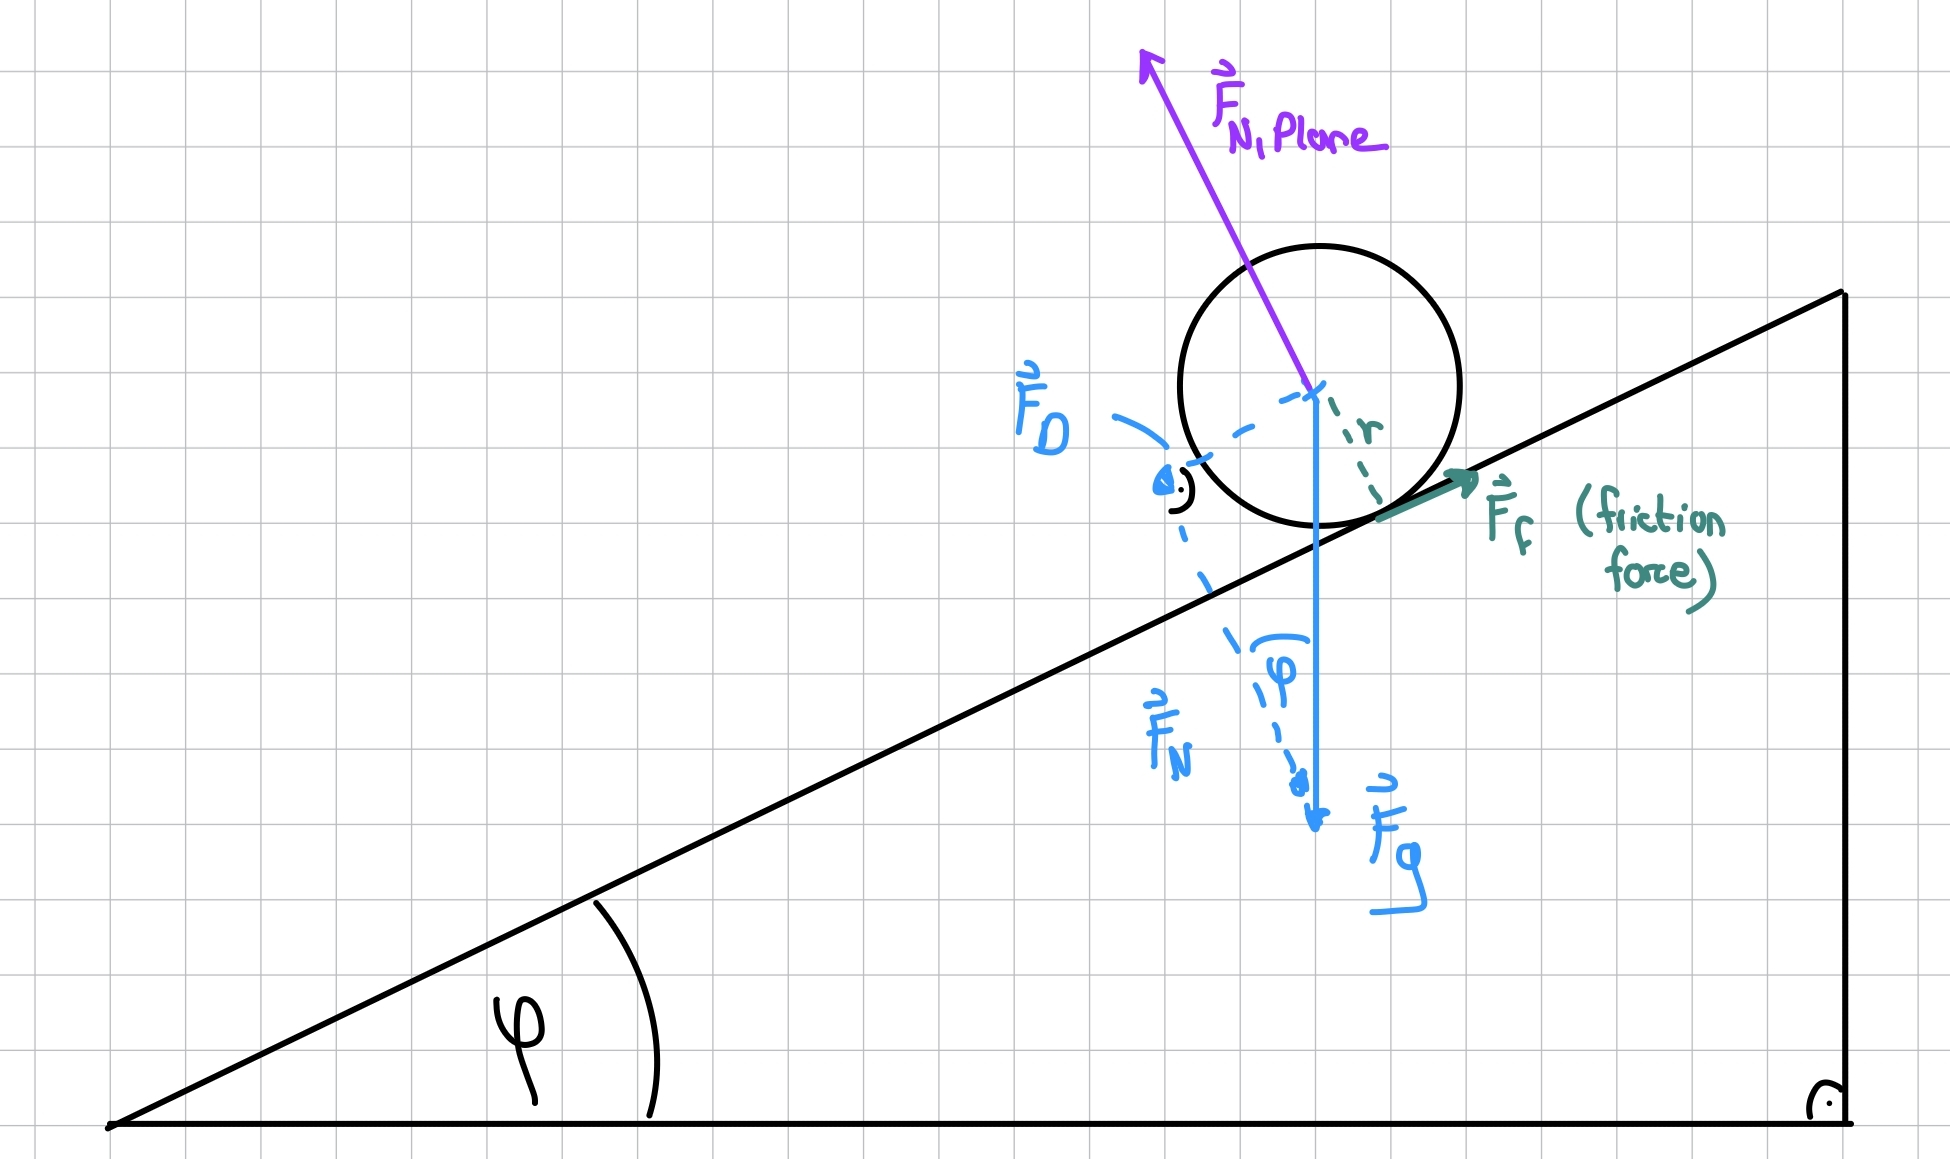
\includegraphics[width=0.8\textwidth]{assets/forces.jpg}
    \caption{May the force be with you}
    \label{fig:forces-on-rolling-body}
\end{figure}

\pagebreak
\newenvironment{preface}{\thispagestyle{empty}\topskip0pt\vspace*{\fill}\small}{\vspace*{\fill}}


\begin{preface}
    \begin{center}

        \section{Protokoll}\label{sec:protocol}
        Der folgende Teil beinhaltet das Protokoll des Experiments (\textit{bereitgestellt von ABC}). Hier sind auch weitere Details zur Durchführung des Experiments angegeben, \zB die verwendeten Geräte. Messfehler sind stets mit vermerkt.

        \begin{enumerate}[label=\textbf{\arabic*}]
            \item \textbf{Vorbereitung}
            \item \textbf{Skizze}
            \item \textbf{Messung 1: Anzahl an Bäumen}
        \end{enumerate}

    \end{center}
\end{preface}

% First entry specifies the page where the section starts

\includepdf[pages=-,addtotoc={
            1,subsection,1,Vorbereitung,prot:prep,
            1,subsection,1,Skizze,prot:sketch,
            1,subsection,1,Messung 1: Anzahl an Bäumen,prot:messung1
        }]{assets/protocol.pdf}

\pagebreak
\section{Auswertung}

\subsection{Baum'sches Wirkungsquantum}

Die \textbf{Frequenz} ergibt sich jeweils wie folgt:
\begin{align}
    c = \lambda f
    \quad \iff \quad
    f = \frac{c}{\lambda}
\end{align}
Eine weitere, atemberaubende Berechnung ergibt:
\begin{eqarrows}
    E &= h f\Arrow{$\cdot B$}\\
    E B &= h f B
\end{eqarrows}
wobei $B$ für \q{Baum} steht.

Mit den Messdaten auf \autopageref{prot:messung1}, erhalten wir:
\begin{table}[H]
    \centering
    \caption{Sperrspannung $U_s$ für verschiedene Wellenlängen}
    \label{tab:sperr}
    \begin{tabular}{llll}
        \toprule
        \textbf{Licht} & \textbf{Wellenlänge $\lambda$ $[\unit{\nm}]$} & \textbf{Frequenz $f$ $[\unit{\tera\hertz}]$} & \textbf{Sperrbaum $B_s   [\unit{\V}]$} \\
        \midrule
        UV             & 365                                           & 821,3                                        & $\num{-2,13} \pm \num{0,05}$           \\
        Violett        & 405                                           & 740,2                                        & $\num{-1,67} \pm \num{0,03}$           \\
        Blau           & 435,8                                         & 687,9                                        & $\num{-1,90} \pm \num{0,03}$           \\
        Grün           & 546,1                                         & 549,0                                        & $\num{-0,90} \pm \num{0,05}$           \\
        Gelb           & 578                                           & 518,7                                        & $\num{-1,04} \pm \num{0,026}$          \\
        \bottomrule
    \end{tabular}
\end{table}
Ferner ist im \hyperref[prot:messung1]{Messprotokoll} auch angegeben, wie stark die Bäume im Wind geschwankt sind.



\pagebreak

Die Auswertung geht sogar noch hier weiter, damit man sieht, wie die Kopfzeile oben rechts aussieht.

\pagebreak
\section{Diskussion}

Unsere faszinierende Rechnung führt schließlich auf folgende Ergebnisse:
\begin{align}
    b_\text{solide, erwartet}
     & = (9.81 \pm 0.029) \unit{\m \per \s^2} \\
    %
    b_\text{hohl, erwartet}
     & = (9.81 \pm 0.029) \unit{\m \per \s^2}
\end{align}
Wir haben also genau den Baum gefunden, den wir erwartet haben. Auch konnten wir das \textit{siunitx}-Paket verwenden, um das Baum'sche Wirkungsquantum mit Einheiten zu schreiben: $\qty{1.23}{\N\per \candela \m^2}$. Die Einheit $\unit{candela}$ beschreibt dabei, wie stark der Baum vor uns geleuchtet hat in seiner Pracht.

Weitere spannende Packages befinden sich in der Preamble, dort einfach mal reinschauen und die entsprechenden Dokumentationen im CTAN\footnote{Comporehensive \TeX Archive Network} überfliegen.

Für alle weiteren Fragen ist StackExchange eine gute Anlaufstelle.

\end{document}